\scanpage{85}
\mspage{- 538 -}

\begin{center}
TABLE DES MATIERES
\end{center}

\noindent AVANT-PROPOS \dotfill

\noindent INTRODUCTION\dotfill

\noindent CHAPITRE \unsure{O|0} .- Préliminaires\dotfill

\noindent\quad \S\ 1. Foncteurs représentables\dotfill

\noindent\qquad 1.1. Foncteurs représentables\dotfill

\noindent\qquad 1.2. Produits fibrés dans une catégorie\dotfill

\noindent\qquad 1.3. Changement de base\dotfill

\noindent\qquad 1.4. Noyaux ; morphisme diagonal\dotfill

\noindent\qquad 1.5. Foncteurs adjoints\dotfill

\noindent\qquad 1.6. Structures algébriques dans les catégories\dotfill

\noindent\qquad 1.7. Morphismes fonctoriels représentables\dotfill

\noindent\quad \S\ 2. Compléments de topologie\dotfill

\noindent\qquad 2.1. Espaces irréductibles\dotfill

\noindent\qquad 2.2. Espaces localement noethériens\dotfill

\noindent\qquad 2.3. Ensembles quasi-constructibles et ensembles constructibles\dotfill

% Left marginal hook and separate lower dash; question-mark function uncertain.
\margin{\figure{\handwritten{\unsure{%
\begin{tikzpicture}[x=0.1mm,y=0.1mm]
\draw[line width=0.35pt] (0,68)
 .. controls (10,72) and (21,73) .. (23,66)
 .. controls (26,57) and (19,40) .. (16,28)
 .. controls (13,18) and (13,20) .. (20,19)
 .. controls (25,18) and (27,22) .. (31,20);
\draw[line width=0.45pt] (38,0) .. controls (41,1) and (44,1) .. (47,0);
\end{tikzpicture}%
}}}}
% The deletion macros record state; the path preserves the observed connected cancellation.
\figure{%
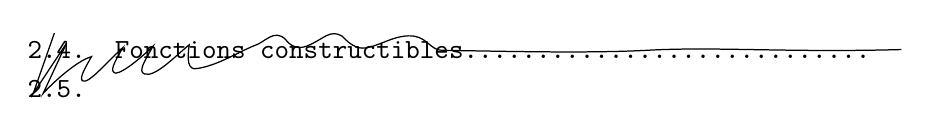
\begin{tikzpicture}[x=0.0008\linewidth,y=0.1mm]
\node[anchor=base west,inner sep=0pt,font=\ttfamily] at (0,0)
 {\deleted{2.4. Fonctions constructibles}\deleted{\mbox{............................}}};
\node[anchor=base west,inner sep=0pt,font=\ttfamily] at (0,-50) {\deleted{2.5.}};
\handwritten{\draw[line width=0.45pt]
 (36,32) -- (8,-45) -- (52,19) -- (21,-45)
 .. controls (28,-37) and (63,-4) .. (85,2)
 .. controls (78,-10) and (67,-27) .. (74,-29)
 .. controls (82,-32) and (106,-4) .. (126,13)
 .. controls (115,-6) and (108,-17) .. (117,-19)
 .. controls (128,-18) and (153,3) .. (166,15)
 .. controls (155,-4) and (146,-17) .. (155,-20)
 .. controls (169,-25) and (198,5) .. (214,17)
 .. controls (211,-2) and (212,-16) .. (225,-13)
 .. controls (252,-9) and (279,8) .. (300,16)
 .. controls (314,20) and (326,38) .. (341,24)
 .. controls (349,13) and (361,11) .. (373,17)
 .. controls (392,25) and (400,37) .. (416,28)
 .. controls (427,16) and (439,10) .. (451,14)
 .. controls (468,17) and (488,31) .. (511,28)
 .. controls (529,25) and (533,10) .. (548,10)
 .. controls (626,9) and (735,6) .. (817,10)
 .. controls (907,15) and (1001,7) .. (1154,11);}
\end{tikzpicture}%
}

\noindent\qquad 2.4. Ensembles constructibles dans les espaces noethériens

\noindent\qquad 2.5? Fonctions constructibles\dotfill

\noindent\qquad 2.6. Parties très denses d'un espace topologique\dotfill

\noindent\qquad 2.7. Quasi-homéomorphismes\dotfill

\noindent\qquad 2.8. Espaces de Jacobson\dotfill

\noindent\qquad 2.9. Espace sobre associé à un espace topologique\dotfill

\noindent\qquad 2.10.Applications ouvertes en un point \dotfill

\noindent\quad \S\ 3. Compléments sur les faisceaux\dotfill

\noindent\qquad 3.1. Faisceaux à valeurs dans une catégorie\dotfill

\noindent\qquad 3.2. Préfaisceaux sur une base d'ouverts\dotfill

\noindent\qquad 3.3. Recollement de faisceaux\dotfill

\noindent\qquad 3.4. Images directes de préfaisceaux\dotfill

\noindent\qquad 3.5. Images réci\deleted{\unsure{r}}p\deleted{p}roque\unsure{s|\deleted{s}s} de préfaisceaux\dotfill

\noindent\qquad 3.6. Faisceaux simples et faisceaux localement simples\dotfill

\noindent\qquad 3.7. Images réciproques de faisceaux de groupes ou d'anneaux\dotfill

% archive sheet number: 84
